\documentclass{../inc/mybib}

% \graphicspath{{../assets/images/}}
\title{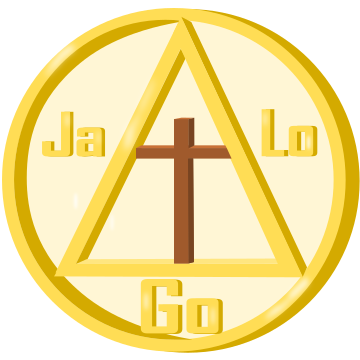
\includegraphics[height=48pt]{../assets/images/logo.png} \\Das Licht}
\author{Lothar Schmid}
\begin{document}
\maketitle
\section{Begrüssung}

Ich möchte euch alle recht herzlich zu diesem besonderen Gottesdienst begrüssen. Schön das so viele gekommen sind, um unserem Herrn zu Danken ihn zu Loben und zu Preisen.

Auch möchte ich Philipp begrüßen, der den Weg von Zürich über Bern hier gemacht hat, um uns das Wort des Herrn zu verkünden. 

\noindent
\beten{} und anschließend singen wir zusammen das Lied

\noindent
\lied{In der Nacht von Betlehem}.

\section{Ankündigungen}
\begin{itemize}
    \item \green{Bibel und Gebetsabend:} Do 19.12.2024 20:00Uhr mit Norbert Lieth ab Römer 11:33-36
    \item \green{Nächster Gottesdienst:} So 22.12.2024 15:00Uhr mit Fredy Peter
    \item \green{Diverses:} -
    \item \green{Die Kollekte:} Die Kollekte geht an den Mitternachtsruf und wird dort für die Missionsarbeit in der Welt eingesetzt.
\end{itemize}

\section{ Input }
\begin{spacing}{1.5}
\subsection{ Das Licht }

Viel wird über Jesus als das Licht geschrieben und geredet. Vor allem in dieser aktuellen Zeit. Weihnachten ist ein Fest des Lichtes. Häuser werden geschmückt, Bäume mit Lampen behangen. In Gärten kitschige leuchtende Tiere und Figuren aufgestellt. Die Menschen freuen sich an diesen Lichter. Das Licht gibt uns Sicherheit. Nur dunkle Gestalten vermeiden das Licht und drucken sich durch die finsteren Gassen um etwas anzustellen. 

In der ganzen Bibel ist das Licht ein Symbol von Gerechtigkeit und Offenheit. Gott sagt zu David, als er ihm sein Fehler mit Batseba aufzeigt folgendes:

\begin{bibeltext}{SCHL}{2Sam}{12:12}
Denn du hast es heimlich getan; ich aber will diese Sache vor ganz Israel und am helllichten Tag tun!
\end{bibeltext}

Auch unsere Taten ob gut oder schlecht, werden eines Tages von Gott an das helle Licht gebracht.
Durch Jesu Blut wurden wir reingewaschen und Jesus ist unsere Leuchte auf unserem Weg hier auf Erden. Er ist das ewige Licht. Und weil wir durch Jesus errettet wurden, sollen wir das Licht, dass wir von ihm empfangen haben, weiter tragen und unseren Mitmenschen damit ihr Weg erleuchten.

Zu diesem Text möchte ich euch aus dem Evangelium von Johannes Kapitel 1:1 - 14 vorlesen.
Und dann passend dazu den Psalm 47. Danach singen wir das Lied Macht hoch die Tür.

\end{spacing}

\lied{Macht hoch die Tür}

\section{Predigt}
\green{Schriftlesung}

Danach gebe ich das Wort an Philipp weiter.

\textbf{Nach der Predigt}

Danken für die Predigt

\section{Abschluss}

Jetzt wollen wir Gott mit dem Lied \lied{Tochter Zion freue dich} danken.


Vielen Dank für eure Teilnahme und das Gebet. Im Anschluss seid ihr zu Kaffee und guten Gesprächen eingeladen.
\beten{}

\begin{bibeltext}{SCHL}{Phil}{4:20.23}
Unser Gott und Vater aber sei die Herrlichkeit von Ewigkeit zu Ewigkeit!
Die Gnade des Herrn Jesus Christus sei mit eurem Geist!
\end{bibeltext}

Maranatha Amen
\end{document}